\documentclass[aspectratio=169]{beamer}
\usetheme{metropolis}
\usepackage{graphicx}
\usepackage{listings}
\usepackage{xcolor}
\usepackage{fontawesome5}
\usepackage{tikz}
\usetikzlibrary{shapes.geometric, arrows, positioning}

% Colors
\definecolor{gnarkblue}{RGB}{59, 130, 246}
\definecolor{gnarkgreen}{RGB}{34, 197, 94}
\definecolor{gnarkred}{RGB}{239, 68, 68}
\definecolor{gnarkyellow}{RGB}{250, 204, 21}
\definecolor{gnarkpurple}{RGB}{139, 92, 246}
\definecolor{codebg}{RGB}{30, 30, 46}
\definecolor{codetext}{RGB}{205, 214, 244}

\setbeamercolor{frametitle}{bg=gnarkblue}
\setbeamercolor{progress bar}{fg=gnarkpurple}

% Code listings style
\lstset{
    basicstyle=\ttfamily\scriptsize\color{codetext},
    backgroundcolor=\color{codebg},
    keywordstyle=\color{gnarkpurple},
    stringstyle=\color{gnarkgreen},
    commentstyle=\color{gray},
    breaklines=true,
    frame=single,
    rulecolor=\color{gnarkblue},
    showstringspaces=false
}

\title{\textbf{internal/smt}}
\subtitle{Formal Verification for gnark Circuits with SMT Solvers}
\author{gnark Team}
\date{}
\institute{Consensys}

\begin{document}

\maketitle

% ============================================================================
\section{The Problem}

\begin{frame}{Circuit Bugs Are Expensive}
    \begin{columns}
        \begin{column}{0.5\textwidth}
            \textbf{\large Common ZK Circuit Vulnerabilities:}
            \begin{itemize}
                \item \textcolor{gnarkred}{\faExclamationTriangle} Under-constrained variables
                \item \textcolor{gnarkred}{\faExclamationTriangle} Missing range checks
                \item \textcolor{gnarkred}{\faExclamationTriangle} Unconstrained hint outputs
                \item \textcolor{gnarkred}{\faExclamationTriangle} Redundant constraints (inefficiency)
            \end{itemize}

            \vspace{1em}
            \textbf{The Challenge:}\\
            Manual review doesn't scale\\
            Testing can miss edge cases
        \end{column}
        \begin{column}{0.5\textwidth}
            \begin{tikzpicture}[scale=0.9]
                \node[draw, rounded corners, fill=gnarkblue!20, minimum width=4cm, minimum height=1cm] (circuit) at (0,3) {\textbf{Your Circuit}};
                \node[draw, rounded corners, fill=gnarkgreen!20, minimum width=4cm, minimum height=1cm] (compile) at (0,1.5) {gnark Compiler};
                \node[draw, rounded corners, fill=gnarkyellow!20, minimum width=4cm, minimum height=1cm] (constraints) at (0,0) {PlonK Constraints};
                \node[draw, rounded corners, fill=gnarkred!20, minimum width=4cm, minimum height=1cm] (bugs) at (0,-1.5) {\faQuestion~Are they sound?};

                \draw[->, thick] (circuit) -- (compile);
                \draw[->, thick] (compile) -- (constraints);
                \draw[->, thick, dashed, gnarkred] (constraints) -- (bugs);
            \end{tikzpicture}
        \end{column}
    \end{columns}
\end{frame}

% ============================================================================
\section{The Solution}

\begin{frame}{Introducing \texttt{internal/smt}}
    \begin{center}
        \textbf{\Large Formal Verification of \underline{Actual} Compiled Constraints}
    \end{center}

    \vspace{1em}

    \begin{columns}
        \begin{column}{0.5\textwidth}
            \textbf{\textcolor{gnarkgreen}{\faCheckCircle} What it does:}
            \begin{itemize}
                \item Extracts real PlonK constraints from gnark
                \item Exports to SMT solver formats
                \item Detects under-constrained circuits
                \item Generates beautiful reports
            \end{itemize}
        \end{column}
        \begin{column}{0.5\textwidth}
            \textbf{\textcolor{gnarkblue}{\faCogs} Key Insight:}

            \vspace{0.5em}
            Don't verify hand-written approximations.

            \vspace{0.5em}
            Verify the \textit{actual constraints} that the gnark compiler produces!
        \end{column}
    \end{columns}

    \vspace{1em}
    \begin{center}
        \colorbox{codebg}{\textcolor{codetext}{\texttt{qL*xa + qR*xb + qO*xc + qM*(xa*xb) + qC = 0}}}
    \end{center}
\end{frame}

% ============================================================================
\begin{frame}[fragile]{Simple API}
\begin{lstlisting}[language=Go,escapechar=|]
// Compile your circuit and analyze it in 5 lines
circuit := &MyCircuit{}
opts := smt.DefaultCompileOptions()
opts.TestName = "MyCircuit"

result, err := smt.CompileCircuit(circuit, opts)
if err != nil {
    log.Fatal(err)
}

// Print analysis results
result.PrintSummary()

// Generate HTML report
result.WriteReportToFile("report.html", "MyCircuit")

// Export for cvc5 verification
result.WriteToFile("verify_mycircuit.cpp")
\end{lstlisting}
\end{frame}

% ============================================================================
\section{Features}

\begin{frame}{Feature 1: Static Analysis}
    \textbf{\large Instant Soundness Checks (No SMT Solver Required)}

    \vspace{1em}

    \begin{columns}
        \begin{column}{0.5\textwidth}
            \textbf{Detects:}
            \begin{itemize}
                \item \textcolor{gnarkred}{\faBug} Unused variables
                \item \textcolor{gnarkred}{\faBug} Trivial/impossible constraints
                \item \textcolor{gnarkred}{\faBug} Missing range checks on limbs
                \item \textcolor{gnarkred}{\faBug} Unbounded secret variables
                \item \textcolor{gnarkred}{\faBug} Under-constrained hint outputs
                \item \textcolor{gnarkred}{\faBug} Unconstrained public outputs
            \end{itemize}
        \end{column}
        \begin{column}{0.5\textwidth}
            \textbf{Pattern Recognition:}
            \begin{itemize}
                \item Decomposition patterns
                \item Inverse check patterns
                \item Range constraint detection
                \item Log-derivative argument detection
            \end{itemize}

            \vspace{1em}
            \colorbox{gnarkgreen!20}{\textcolor{gnarkgreen}{\faRocket~Runs in milliseconds}}
        \end{column}
    \end{columns}
\end{frame}

% ============================================================================
\begin{frame}{Feature 2: SMT Solver Export}
    \textbf{\large Two Export Formats for cvc5}

    \vspace{1em}

    \begin{columns}
        \begin{column}{0.5\textwidth}
            \textbf{\textcolor{gnarkblue}{\faCode} C++ API Export}
            \begin{itemize}
                \item Full cvc5 C++ integration
                \item Ready-to-compile verification code
                \item Helper functions included
                \item Test scaffolding generated
            \end{itemize}

            \vspace{0.5em}
            \colorbox{codebg}{\scriptsize\texttt{\textcolor{codetext}{g++ -std=c++17 verify.cpp -lcvc5}}}
        \end{column}
        \begin{column}{0.5\textwidth}
            \textbf{\textcolor{gnarkpurple}{\faFile*} SMT-LIB2 Export}
            \begin{itemize}
                \item Standard SMT format
                \item QF\_FF logic (finite fields)
                \item Works with any compatible solver
                \item Human-readable formulas
            \end{itemize}

            \vspace{0.5em}
            \colorbox{codebg}{\scriptsize\texttt{\textcolor{codetext}{cvc5 verify.smt2}}}
        \end{column}
    \end{columns}

    \vspace{1em}
    \begin{center}
        \textbf{Prove properties like:}\\
        ``Variable X is uniquely determined by inputs''\\
        ``Removing constraint N allows invalid witnesses''
    \end{center}
\end{frame}

% ============================================================================
\begin{frame}{Feature 3: Source Location Tracking}
    \textbf{\large Know Exactly Where Issues Originate}

    \vspace{1em}

    \begin{itemize}
        \item Integrates with gnark's profiling system
        \item Maps constraints back to your Go source code
        \item Full stack traces for complex circuits
        \item Filters out internal gnark code automatically
    \end{itemize}

    \vspace{1em}

    \begin{center}
    \colorbox{codebg}{
    \begin{minipage}{0.7\textwidth}
    \color{codetext}\ttfamily\scriptsize
    [CRITICAL] missing-range-check\\
    ~~ Variable: limb\_0\\
    ~~ Location: \textcolor{gnarkpurple}{mycircuit.go:47}\\
    ~~ Stack trace:\\
    ~~~~ $\rightarrow$ MyCircuit.Define at mycircuit.go:47\\
    ~~~~~~ api.ToBinary at api.go:123
    \end{minipage}
    }
    \end{center}
\end{frame}

% ============================================================================
\begin{frame}{Feature 4: Beautiful Reports}
    \textbf{\large Multiple Output Formats}

    \vspace{0.5em}

    \begin{columns}
        \begin{column}{0.33\textwidth}
            \textbf{\faTerminal~Terminal}
            \begin{itemize}
                \item ANSI colors
                \item Progress indicators
                \item Quick feedback
            \end{itemize}
        \end{column}
        \begin{column}{0.33\textwidth}
            \textbf{\faHtml5~HTML}
            \begin{itemize}
                \item Dark theme UI
                \item Interactive elements
                \item Shareable reports
            \end{itemize}
        \end{column}
        \begin{column}{0.33\textwidth}
            \textbf{\faFileCode~JSON}
            \begin{itemize}
                \item Machine-readable
                \item CI/CD integration
                \item Structured data
            \end{itemize}
        \end{column}
    \end{columns}

    \vspace{1em}

    \begin{center}
    \colorbox{codebg}{
    \begin{minipage}{0.8\textwidth}
    \color{codetext}\ttfamily\scriptsize
    \textcolor{gnarkgreen}{[PASS]} All internal variables are uniquely determined\\
    \textcolor{gnarkgreen}{[PASS]} Constraint 42: multiplication with non-zero constant\\
    \textcolor{gnarkyellow}{[WARN]} Secret variable 'k' has no apparent range constraint\\
    \textcolor{gnarkred}{[FAIL]} Hint output 'quotient' appears in only one constraint
    \end{minipage}
    }
    \end{center}
\end{frame}

% ============================================================================
\section{How It Works}

\begin{frame}{Architecture}
    \begin{center}
    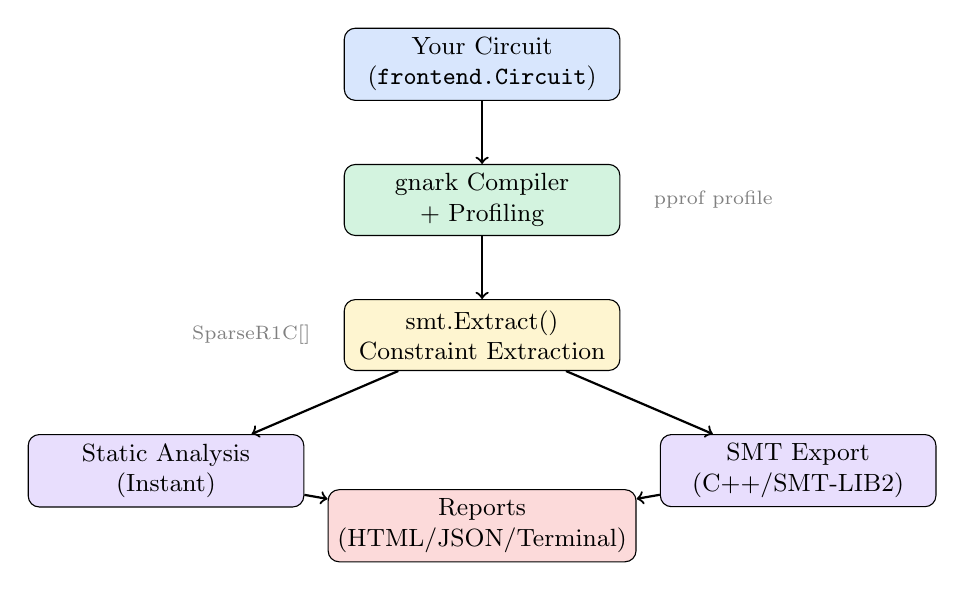
\begin{tikzpicture}[
        node distance=0.8cm,
        box/.style={draw, rounded corners, minimum width=3.5cm, minimum height=0.9cm, align=center, font=\small},
        arrow/.style={->, thick}
    ]
        % Input
        \node[box, fill=gnarkblue!20] (circuit) {Your Circuit\\(\texttt{frontend.Circuit})};

        % Compile
        \node[box, fill=gnarkgreen!20, below=of circuit] (compile) {gnark Compiler\\+ Profiling};

        % Extract
        \node[box, fill=gnarkyellow!20, below=of compile] (extract) {smt.Extract()\\Constraint Extraction};

        % Analysis branches
        \node[box, fill=gnarkpurple!20, below left=0.8cm and 0.5cm of extract] (static) {Static Analysis\\(Instant)};
        \node[box, fill=gnarkpurple!20, below right=0.8cm and 0.5cm of extract] (export) {SMT Export\\(C++/SMT-LIB2)};

        % Output
        \node[box, fill=gnarkred!20, below=1.5cm of extract] (report) {Reports\\(HTML/JSON/Terminal)};

        % Arrows
        \draw[arrow] (circuit) -- (compile);
        \draw[arrow] (compile) -- (extract);
        \draw[arrow] (extract) -- (static);
        \draw[arrow] (extract) -- (export);
        \draw[arrow] (static) -- (report);
        \draw[arrow] (export) -- (report);

        % Labels
        \node[right=0.3cm of compile, font=\scriptsize\color{gray}] {pprof profile};
        \node[left=0.3cm of extract, font=\scriptsize\color{gray}] {SparseR1C[]};
    \end{tikzpicture}
    \end{center}
\end{frame}

% ============================================================================
\begin{frame}{PlonK Constraint Format}
    \textbf{\large Understanding What Gets Verified}

    \vspace{1em}

    Every gnark constraint compiles to:

    \begin{center}
        \colorbox{gnarkblue!10}{
            \Large $q_L \cdot x_a + q_R \cdot x_b + q_O \cdot x_c + q_M \cdot (x_a \cdot x_b) + q_C = 0$
        }
    \end{center}

    \vspace{1em}

    \begin{columns}
        \begin{column}{0.5\textwidth}
            \textbf{Variables:}
            \begin{itemize}
                \item $x_a, x_b, x_c$ -- Wire indices
                \item Public, Secret, or Internal
            \end{itemize}
        \end{column}
        \begin{column}{0.5\textwidth}
            \textbf{Coefficients:}
            \begin{itemize}
                \item $q_L, q_R, q_O$ -- Linear terms
                \item $q_M$ -- Multiplication term
                \item $q_C$ -- Constant term
            \end{itemize}
        \end{column}
    \end{columns}

    \vspace{1em}

    \begin{center}
        \textcolor{gnarkgreen}{\faCheckCircle}~The smt package extracts \textit{exactly} these values from compiled circuits
    \end{center}
\end{frame}

% ============================================================================
\section{Use Cases}

\begin{frame}[fragile]{Use Case 1: CI/CD Integration}
    \textbf{\large Automated Soundness Checks in Your Pipeline}

    \vspace{0.5em}

\begin{lstlisting}[language=Go,escapechar=|]
func TestCircuitSoundness(t *testing.T) {
    circuit := &MyCircuit{}
    result, _ := smt.CompileCircuit(circuit,
                     smt.DefaultCompileOptions())

    // Run static analysis
    analysis := result.Analyze("MyCircuit")

    // Fail on critical issues
    if analysis.HasCritical() {
        analysis.Print(os.Stdout)
        t.Fatal("Circuit has critical soundness issues")
    }
}
\end{lstlisting}
\end{frame}

% ============================================================================
\begin{frame}{Use Case 2: Security Audits}
    \textbf{\large Generate Artifacts for Auditors}

    \vspace{1em}

    \begin{columns}
        \begin{column}{0.5\textwidth}
            \textbf{What auditors get:}
            \begin{itemize}
                \item Complete constraint listing
                \item Automatic issue detection
                \item Source location mapping
                \item Exportable verification code
            \end{itemize}
        \end{column}
        \begin{column}{0.5\textwidth}
            \textbf{Audit workflow:}
            \begin{enumerate}
                \item Run static analysis
                \item Review flagged issues
                \item Export to cvc5 for deep checks
                \item Generate report for docs
            \end{enumerate}
        \end{column}
    \end{columns}

    \vspace{1em}

    \begin{center}
    \colorbox{codebg}{
    \begin{minipage}{0.75\textwidth}
    \color{codetext}\ttfamily\scriptsize
    go run audit\_tool.go -circuit=MyCircuit \\
    ~~~~-html=audit\_report.html \\
    ~~~~-cpp=verify\_constraints.cpp
    \end{minipage}
    }
    \end{center}
\end{frame}

% ============================================================================
\begin{frame}{Use Case 3: Development Debugging}
    \textbf{\large Find Issues Before They Become Vulnerabilities}

    \vspace{1em}

    \begin{columns}
        \begin{column}{0.5\textwidth}
            \textbf{During development:}
            \begin{itemize}
                \item Quick feedback loop
                \item Catch under-constraints early
                \item Understand constraint patterns
                \item Verify hint outputs
            \end{itemize}
        \end{column}
        \begin{column}{0.5\textwidth}
            \textbf{Example output:}

            \vspace{0.5em}
            \colorbox{codebg}{
            \begin{minipage}{\textwidth}
            \color{codetext}\ttfamily\tiny
            Linear constraints: 42\\
            Multiplication constraints: 18\\
            Decomposition (a+k*b=c): 8\\
            Inverse checks (a*b=1): 4\\
            \\
            \textcolor{gnarkred}{[CRITICAL]} Hint output 'inv'\\
            never constrained!
            \end{minipage}
            }
        \end{column}
    \end{columns}

    \vspace{1em}

    \begin{center}
        \colorbox{gnarkgreen!20}{\textcolor{gnarkgreen}{\faLightbulb~Catch the bug in development, not in production}}
    \end{center}
\end{frame}

% ============================================================================
\section{Getting Started}

\begin{frame}[fragile]{Quick Start}
\begin{lstlisting}[language=Go,escapechar=|]
package main

import (
    "log"
    "github.com/consensys/gnark/internal/smt"
)

func main() {
    circuit := &MyCircuit{} // Your circuit

    // Compile and analyze
    opts := smt.DefaultCompileOptions()
    opts.TestName = "MyCircuit"
    opts.WithProfiling = true // Enable source tracking

    result, err := smt.CompileCircuit(circuit, opts)
    if err != nil { log.Fatal(err) }

    // Generate report
    result.WriteReportToFile("analysis.html", "MyCircuit")
}
\end{lstlisting}
\end{frame}

% ============================================================================
\begin{frame}{cvc5 Integration}
    \textbf{\large Running SMT Verification}

    \vspace{1em}

    \textbf{1. Install cvc5:}
    \begin{center}
        \colorbox{codebg}{\textcolor{codetext}{\texttt{brew install cvc5}}}~~or~~\colorbox{codebg}{\textcolor{codetext}{\texttt{apt install cvc5}}}
    \end{center}

    \vspace{1em}

    \textbf{2. Compile the generated C++:}
    \begin{center}
        \colorbox{codebg}{\textcolor{codetext}{\texttt{g++ -std=c++17 verify.cpp -lcvc5 -o verify}}}
    \end{center}

    \vspace{1em}

    \textbf{3. Run verification:}
    \begin{center}
        \colorbox{codebg}{\textcolor{codetext}{\texttt{./verify}}}
    \end{center}

    \vspace{1em}

    \begin{center}
        \textcolor{gnarkgreen}{\faCheckCircle}~Tests constraint satisfiability\\
        \textcolor{gnarkgreen}{\faCheckCircle}~Verifies variable uniqueness\\
        \textcolor{gnarkgreen}{\faCheckCircle}~Checks constraint necessity
    \end{center}
\end{frame}

% ============================================================================
\section{Summary}

\begin{frame}{Why Use \texttt{internal/smt}?}
    \begin{columns}
        \begin{column}{0.5\textwidth}
            \textbf{\large \textcolor{gnarkgreen}{\faCheckCircle} Benefits:}

            \vspace{0.5em}

            \begin{itemize}
                \item \textbf{Real constraints} -- Not approximations
                \item \textbf{Instant feedback} -- Static analysis in ms
                \item \textbf{Formal proofs} -- SMT solver integration
                \item \textbf{Source tracking} -- Know where bugs are
                \item \textbf{Beautiful reports} -- HTML, JSON, Terminal
                \item \textbf{CI/CD ready} -- Automated testing
            \end{itemize}
        \end{column}
        \begin{column}{0.5\textwidth}
            \textbf{\large \textcolor{gnarkblue}{\faUsers} Who should use it:}

            \vspace{0.5em}

            \begin{itemize}
                \item Circuit developers
                \item Security auditors
                \item QA/Testing teams
                \item Anyone building with gnark
            \end{itemize}

            \vspace{1em}

            \colorbox{gnarkpurple!20}{
            \begin{minipage}{\textwidth}
            \centering
            \textcolor{gnarkpurple}{\faStar~\textbf{Find bugs before attackers do}}
            \end{minipage}
            }
        \end{column}
    \end{columns}
\end{frame}

% ============================================================================
\begin{frame}{}
    \begin{center}
        \Huge \textbf{Questions?}

        \vspace{2em}

        \Large
        \texttt{github.com/consensys/gnark}

        \vspace{1em}

        \normalsize
        \texttt{internal/smt}

        \vspace{2em}

        \textcolor{gnarkblue}{\faGithub}~~\textcolor{gnarkpurple}{\faBook}~~\textcolor{gnarkgreen}{\faComments}
    \end{center}
\end{frame}

\end{document}
